\documentclass[12pt]{extarticle}

% meta
\title{Отчет о практическом задании \\ <<Градиентные методы обучения линейных моделей>>.\\[6mm] \large Практикум 317 группы, ММП ВМК МГУ.}
\author{Алексеев Илья Алексеевич.}
\date{Ноябрь 2022.}

\usepackage[warn]{mathtext}
\usepackage[T2A]{fontenc}			% кодировка
\usepackage[utf8]{inputenc}			% кодировка исходного текста
\usepackage[english,russian]{babel}	% локализация и переносы
\usepackage{indentfirst}
\usepackage{csquotes}
\usepackage[bibstyle=gost-numeric, sorting=none]{biblatex}
\addbibresource{biblio.bib}

% page settings
\usepackage[left=1.8cm,right=1.8cm,
    top=1.8cm,bottom=1.8cm,bindingoffset=0cm]{geometry}

\usepackage{graphicx, hyperref, xcolor}
\hypersetup{
    colorlinks=true,
    linkcolor=black,
    filecolor=magenta, 
    urlcolor=blue,
    citecolor=olive,
    pdftitle={GD},
    pdfpagemode=FullScreen,
    linktoc=all
    }

\usepackage{wrapfig,caption}

% figures
\usepackage{caption}
\usepackage{subcaption}
\usepackage{floatrow}
\floatsetup{heightadjust=object}

% math
\usepackage{amsmath,amsfonts,amssymb,amsthm,mathtools,esint,eucal}

\newcommand{\R}{\mathbb{R}}
\let\P\relax
\newcommand{\P}{\mathbb{P}}
\let\L\relax
\newcommand{\L}{\mathcal{L}}
\newcommand{\eps}{\varepsilon}
\DeclareMathOperator{\sign}{\text{sign}}
\DeclareMathOperator{\tf}{\text{tf}}
\DeclareMathOperator{\idf}{\text{idf}}
\DeclareMathOperator{\df}{\text{df}}
\DeclareMathOperator{\N}{\text{Norm}}
\let\U\relax
\DeclareMathOperator{\U}{\text{Uniform}}
\DeclareMathOperator{\Exp}{\text{Exp}}

\begin{document}

\maketitle

\tableofcontents

\newpage

\section{Введение.}

Данное практическое задание посвящено исследованию градиентного спуска и стохастического градиентного спуска на примере обучения логистической регрессии в задаче распознавания токсичности текста~\cite{kaggle}. Рассмотрена зависимость сходимости методов от величины шага (learning rate), степени затухания шага и начального приближения весов модели. Для векторизации были использованы методы \texttt{Bag of words} и \texttt{Tf-Idf}. К тексту были применены лемматизация и удаление стоп слов.

\section{Пояснения к задаче.}

\subsection{Бинарная классификация.}

Обучающая выборка $X=\{(x_i,y_i)\}_{i=1}^\ell$, где $x_i\in\R^d,\ y_i\in\mathbb{Y}=\{-1,+1\}$. Линейная модель классификации:
\begin{equation*}
    a(x)=\sign(\langle w,x\rangle).
\end{equation*}
Отступ на $i$-ом объекте: $M_i(w)=y_i\langle w,x_i\rangle$. Сигмоида: $\sigma(z)=1/(1+e^{-z})$. Логарифмическая функция потерь: $\L(M)=-\log(\sigma(M))$, где $\log(x)$ -- натуральный логарифм числа $x$. Функционал эмпирического риска:
\begin{equation*}
    Q(X, w)=-{1\over \ell}\sum_{i=1}^\ell\log(\sigma(y_i\langle w, x_i\rangle)).
\end{equation*}
Производная сигмоиды по весу $w_j$:
\begin{equation*}
    {\partial\over\partial w_j}\sigma(y\langle w, x\rangle)={\partial\over\partial w_j}\left[{1\over1+\exp(-y\langle w, x\rangle)}\right]=-{-yx_j\exp(-y\langle w, x\rangle)\over(1+\exp(-y\langle w, x\rangle))^2}=\sigma(1-\sigma)yx_j.
\end{equation*}
Пусть $\sigma_i=\sigma(y_i\langle w, x_i\rangle)$. Производная по весу $w_j$:
\begin{equation*}
    {\partial\over\partial w_j}Q(X, w)=-{1\over\ell}\sum_{i=1}^\ell{1\over\sigma_i}{\partial\sigma_i\over\partial w_j}=-{1\over\ell}\sum_{i=1}^\ell(1-\sigma_i)y_ix_{ij}
\end{equation*}
Пусть $\sigma\in\R^\ell$ -- вектор с компонентами $\sigma_i$. Пусть вектор $c=a\circ b$ таков, что $c_i=a_ib_i$, где $a,b,c\in\R^\ell$. Тогда градиент функционала эмпирического риска равен
\begin{equation*}
    \nabla_w Q(X, w)=-{1\over \ell}X^T[y\circ(1-\sigma)].
\end{equation*}
Вместе с $L2$-регуляризацией:
\begin{equation}\label{eq:lograd}
    \nabla_w Q(X, w)=-{1\over \ell}X^T[y\circ(1-\sigma)]+\lambda w.
\end{equation}

\subsection{Многоклассовая классификация.}
Обучающая выборка $X=\{(x_i,y_i)\}_{i=1}^\ell$, где $x_i\in\R^d,\ y_i\in\mathbb{Y}=\{1,2,\ldots,K\}$. Линейные модели классификации:
\begin{equation*}
    a_k(x)=\sign(\langle w_k,x\rangle), \quad k=\overline{1,K}.
\end{equation*}
Softmax-преобразование:
\begin{equation*}
    \P(y=j\, |\, x, w)={\exp\langle w_j, x\rangle\over\sum_{k=1}^K\exp\langle w_k, x\rangle}.
\end{equation*}
Минус логарифм правдоподобия является функционалом эмпирического риска:
\begin{equation*}
    Q(X, w)=-{1\over\ell}\sum_{i=1}^\ell\log\P(y_i\, |\, x_i, w).
\end{equation*}
Раскроем логарифм:
\begin{equation*}
    Q(X, w)=-{1\over\ell}\sum_{i=1}^\ell\langle w_{y_i}, x_i\rangle+{1\over\ell}\sum_{i=1}^\ell\log\left(\sum_{k=1}^K\exp\langle w_k, x_i\rangle\right).
\end{equation*}
Пусть $w=(w_1,w_2,\ldots,w_K)\in\R^{d\times K}$ -- матрица весов. Градиентом по вектору $w_p$ будет $p$-ый столбец матрицы $\nabla_wQ$:
\begin{equation*}
    [\nabla_w Q]_p=\nabla_{w_p}Q=-{1\over\ell}\sum_{i:y_i=p}x_i+{1\over\ell}\sum_{i=1}^\ell{x_i\exp\langle w_p, x_i\rangle\over\sum_{k=1}^K\exp\langle w_k,x_i\rangle},\quad p=\overline{1,K}.
\end{equation*}
Вместе $L2$-регуляризацией:
\begin{equation*}
    [\nabla_w Q]_p=-{1\over\ell}\sum_{i:y_i=p}x_i+{1\over\ell}\sum_{i=1}^\ell{x_i\exp\langle w_p, x_i\rangle\over\sum_{k=1}^K\exp\langle w_k,x_i\rangle}+\lambda w_p,\quad p=\overline{1,K}.
\end{equation*}

Пусть $K=2$. Softmax-преобразование:
\begin{gather*}
    \P(y=1\, |\, x, w_1,w_2)={\exp\langle w_1,x\rangle\over\exp\langle w_1,x\rangle+\exp\langle w_2,x\rangle}={1\over1+\exp\langle \underbrace{w_2-w_1}_{\widetilde w},x\rangle}={1\over1+\exp\langle \widetilde w,x\rangle}, \\
    \P(y=2\, |\, x, w_1,w_2)={\exp\langle w_2,x\rangle\over\exp\langle w_1,x\rangle+\exp\langle w_2,x\rangle}={1\over1+\exp\langle \underbrace{w_1-w_2}_{-\widetilde w},x\rangle}={1\over1+\exp\langle -\widetilde w,x\rangle}.
\end{gather*}
Видим, что $\P(y=1\, |\, x,w_1,w_2)=\sigma(-\langle\widetilde w,x\rangle)$, $\P(y=2\, |\, x,w_1,w_2)=\sigma(\langle\widetilde w,x\rangle)$. Если подставить это в функционал эмпирического риска мультиномиальной регрессии, то получим функционал эмпирического риска логистической регрессии для $\mathbb{Y}=\{-1,+1\}$. Значит многоклассовая классификация методом мультиномиальной регрессии при $K=2$ эквивалентна бинарной классификации методом логистической регрессии.

\subsection{Градиентный спуск (GD).}

Градиентным спуском (gradient descent, GD) называют итерационный метод минимизации функционала $f:\R^d\to\R$, при котором $(k+1)$-ый член итерационной последовательности строится следующим образом:
\begin{equation*}
    w^{k+1}=w^k-\eta_k\cdot\nabla f(w^k),\ k=0,1,\ldots
\end{equation*}
Параметрами этого метода являются шаг $\eta_k$ и начальное значение $w_0$. Мы будем рассматривать шаг вида
\begin{equation}\label{eq:gd_step}
    \eta_k={\alpha\over k^\beta},
\end{equation}
где $\alpha>0,\beta>0$ -- параметры. Будем считать, что спуск можно остановить, если было достигнуто предельное число итераций или $|f(w^k)-f(w^{k+1})|<\varepsilon$, где $\varepsilon$ -- некоторое малое число (tolerance).

\subsection{Стохастический градиентный спуск (SGD).}

Стохастический градиентный спуск (stochastic gradient descent, SGD) является модификацией метода градиентного спуска для функционала вида
\begin{equation*}
    Q(w)=\sum_{i=1}^\ell f_i(w).
\end{equation*}
$(k+1)$-ый член итерационной последовательности строится следующим образом:
\begin{align*}
    & I=\{i_1,\ldots,i_b\}\sim\U[0, \ell],\\
    & w^{k+1}=w^k-\eta_k\cdot{1\over b}\sum_{i\in I}\nabla f_i(w^k),\ k=0,1,\ldots
\end{align*}
где $I$ -- выборка уникальных индексов размера $b$ (batch size).

\subsection{Предобработка корпуса и векторизация текста.}

Пусть все слова всех документов (в нашем случае комментариев) образуют множество $\{w_1,w_2,\ldots,w_N\}$. Пусть слово $w$ входит в документ $d$ ровно $\tf(w, d)$ раз. Тогда векторизацией методом \texttt{Bag of words} назовём представление документа $d$ в виде вектора $v(d)\in\R^N$ такого, что
\begin{equation*}
    [v(d)]_i=\tf(w_i, d),\ i=\overline{1,N}. 
\end{equation*}

Пусть слово $w$ встречается ровно в $\df(w)$ документах. Пусть $\idf(w)=\log(n/\df(w))+1$, где $n$ -- общее число документов. Тогда векторизацией методом \texttt{Tf-Idf} назовём представление документа $d$ в виде вектора $v(d)\in\R^N$ такого, что
\begin{equation*}
    [v(d)]_i=\tf(w_i,d)\cdot\idf(w_i),\ i=\overline{1,N}.
\end{equation*}

Лемматизацией текста будем называть приведение каждого его слова к начальной форме. Будем использовать стоп слова из {\texttt{nltk.corpus.stopwords.words('english')}~\cite{nltkstop}}.

\section{Эксперименты.}

Все эксперименты проводились над датасетом контеста Toxic Comment Classification Challenge~\cite{kaggle}. Тренировочный датасет был разбит на обучающую выборку размера 41649 и валидационную выборку размера 10412. Тестовая выборка имеет размер 20676.

\subsection{Предобработка корпуса и векторизация текста.}

Каждый комментарий из обучающей выборки был очищен от всех символов, которые не являются буквами или цифрами, и векторизован методом \texttt{Bag of words}. Чтобы сократить размер вокабулярия и время обучения, были отброшены все слова, доля которых от общего числа слов меньше 0.0001. В результате вокабулярий обучающей выборки сократился с 78694 до 15948 слов. Полученный трансформер был применен к валидационной и тестовой выборкам.

\subsection{Численная проверка градиента.}

Аналитическая формула градиента функции потерь логистической регрессии~\eqref{eq:lograd} была сравнена с численным подсчётом градиента методом конечной разности:
\begin{equation}\label{eq:numgrad}
    {\partial f\over\partial x_i}\approx{f(x+\eps\cdot e_i)-f(x)\over\eps},\ \eps\ll1,\ [e_i]_j=
    \begin{cases}
    1, & i=j,\\
    0, & i\neq j.
    \end{cases}
\end{equation}
Были сгенерированы
\begin{itemize}
    \item выборка $X\in\R^{\ell\times d},\ x_{ij}\sim\Exp(10)$,
    \item ответы $y\in\R^\ell,\ y_i\sim\U\{-1,1\}$,
    \item веса $w\in\R^d,\ w_i\sim\text{N}(0,1)$.
\end{itemize}
На этих данных были найдены градиенты методами \eqref{eq:lograd} и \eqref{eq:numgrad} при $\eps=10^{-3}$ и посчитана $L2$-норма разности между ними $\delta$. Результаты приведены в табл. \ref{tbl:numanal}

\begin{table}[!hbt]
    \centering
    \begin{tabular}{l|l|l}
        $d$ & $\ell$ & $\lg\delta$ \\
        \hline
        50 & 100    & $-10$ \\
        500 & 1000  & $-8$ \\
        5000 & 10000& $-6$ \\
    \end{tabular}
    \caption{Десятичный порядок нормы разницы градиента, посчитанного аналитически \eqref{eq:lograd} и численно \eqref{eq:numgrad}}
    \label{tbl:numanal}
\end{table}

\subsection{Шаг градиентного спуска.}\label{sec:gd_step}

Модель логистической регрессии была обучена методом градиентного спуска для разных значений параметров $\alpha$ и $\beta$, используя правило обновления шага \eqref{eq:gd_step}. По полученной итерационной последовательности весов была посчитана accuracy на валидационной выборке (рис. \ref{fig:step_rough}).

\begin{figure}[!htb]
     \caption{Точность на валидационной выборке (по вертикали) в зависимости от шага градиентного спуска (по горизонтали).}
     \centering
     \begin{subfigure}[t]{0.5\linewidth}
        \caption{Accuracy}
        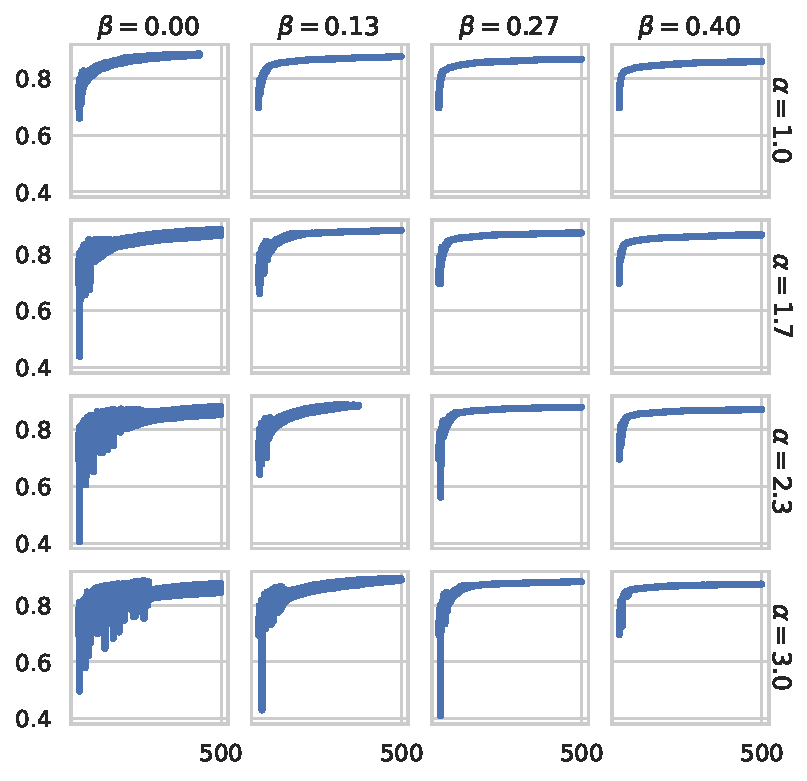
\includegraphics[width=1\linewidth]{pics/accur_step_rough.pdf}
        \label{fig:accur_step_rough}
     \end{subfigure}
     \begin{subfigure}[t]{0.48\linewidth}
        \centering
        \caption{Loss (лог. шкала по горизонтальной оси).}
        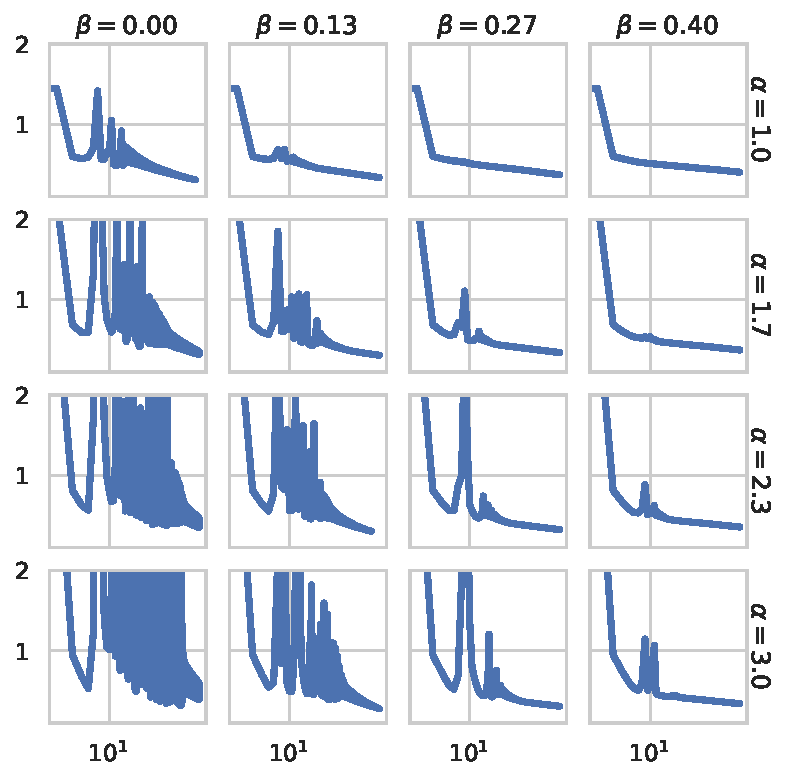
\includegraphics[width=1\linewidth]{pics/loss_step_rough.pdf}
        \label{fig:loss_step_rough}
     \end{subfigure}
     \label{fig:step_rough}
\end{figure}

Заметим, что чем больше параметр $\alpha$, тем большей accuracy удаётся достичь и тем больше метод совершает осцилляций; чем больше параметр $\beta$, тем меньшей accuracy удаётся достичь и тем меньше метод совершает осцилляций.

Из полученных результатов и формулы \eqref{eq:gd_step} следует, что параметр $\alpha$ отвечает за начальную величину шага: если он будет слишком мал, то метод будет сходиться долго, а если -- велик, то метод будет сильно осциллировать. При этом параметр $\beta$ отвечает за угасание шага: если шаг будет угасать слишком быстро, то метод не успеет сойтись, а если -- медленно, то метод не перестанет осциллировать. Значит, оптимальная пара $\alpha$ и $\beta$ способна достичь компромисс между осцилляциями и точностью.

\subsection{Начальное значение градиентного спуска.}\label{sec:w0}

Обучим логистическую регрессию методом градиентного спуска с параметрами $\alpha=1.93,\ \beta=0.21$ и посмотрим на распределение получившихся весов, предварительно убрав выбросы (рис. \ref{fig:weights_distribution}).

Данное распределение можно соотнести с распределением Гаусса, распределением Лапласа и равномерным распределением (рис. \ref{fig:model_weights_distribution}). Гистограмма показывает (рис. \ref{fig:weights_distribution}), что веса сконцентрированы вокруг нуля, но с большим числом выбросов <<вправо>>. Уберем выбросы и построим QQ-графики. По ним видно, что веса хорошо описываются указанными семействами распределений. Вычислим оценки максимального правдоподобия для параметров данных распределений. Сгенерируем начальные значения $w_0$ из полученных распределений.

\begin{figure}[!htb]
     \caption{Распределение весов обученной модели.}
     \centering
     \begin{subfigure}[t]{0.3\linewidth}
        \centering
        \caption{Гистограмма весов.}
        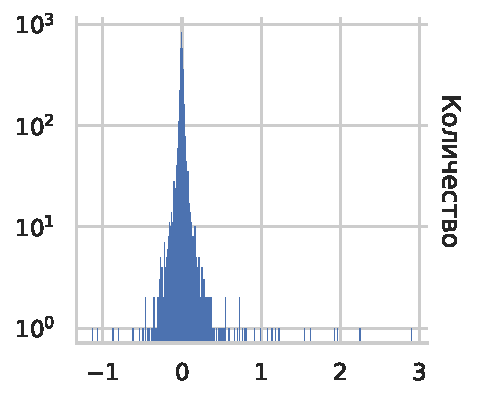
\includegraphics[width=1\linewidth]{pics/weights_distribution.pdf}
        \label{fig:weights_distribution}
     \end{subfigure}
     \begin{subfigure}[t]{0.3\linewidth}
        \centering
        \caption{Квантили распр. Гаусса.}
        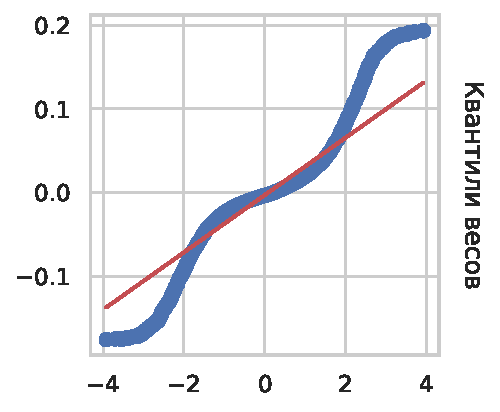
\includegraphics[width=1\linewidth]{pics/weights_norm.pdf}
        \label{fig:weights_norm}
     \end{subfigure}\\
     \begin{subfigure}[t]{0.3\linewidth}
        \centering
        \caption{Квантили распр. Лапласа.}
        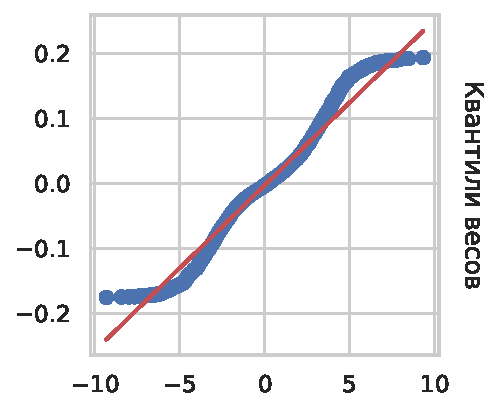
\includegraphics[width=1\linewidth]{pics/weights_lapl.pdf}
        \label{fig:weights_lapl}
     \end{subfigure}
     \begin{subfigure}[t]{0.3\linewidth}
        \centering
        \caption{Квантили равном. распр.}
        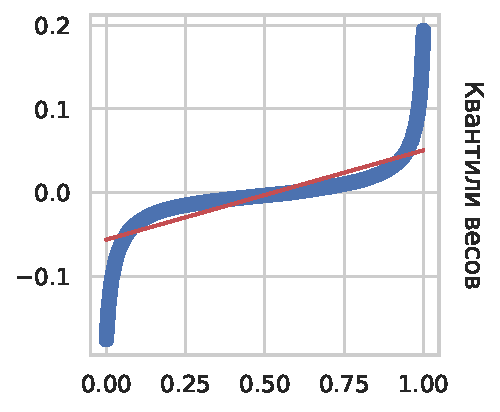
\includegraphics[width=1\linewidth]{pics/weights_unif.pdf}
        \label{fig:weights_unif}
     \end{subfigure}
     \label{fig:model_weights_distribution}
\end{figure}

При обучении модели мы не знаем этих оценок и распределений. Но сейчас у нас не стоит цель придумать эвристику для подбора начальных значений. Мы будем исследовать скорость сходимости градиентного спуска. Были изучены следующие начальные значения: инициализация константой (в том числе $0.0$ и $1.0$), инициализация выборкой из $\U[-1,1]$, инициализация выборкой из $\U[0.2,0.8]$, инициализация выборкой из $\N(0, \sigma_\text{clMML})$, инициализация выборкой из $\N(0.5,\sigma_\text{clMML})$, где $\sigma_\text{clMML}$ -- оценка максимального правдоподобия дисперсии.

% \begin{figure}[!htb]
%      \caption{Точность моделей на валидационной выборке (по вертикали) в зависимости от шага градиентного спуска (по горизонтали). Демонстрация зависимости скорости сходимости градиентного спуска от начального значения.}
%      \centering
%      \begin{subfigure}[t]{0.48\linewidth}
%         \caption{Accuracy}
%         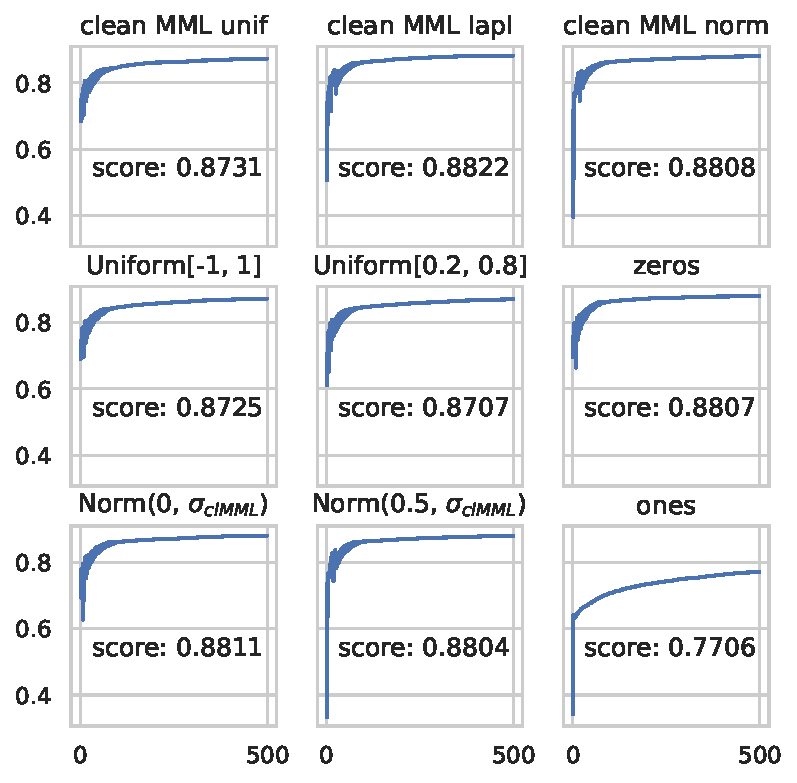
\includegraphics[width=1\linewidth]{pics/init_weights.pdf}
%         \label{fig:init_weights}
%      \end{subfigure}
%      \begin{subfigure}[t]{0.48\linewidth}
%         \centering
%         \caption{Loss (лог. шкала по горизонтальной оси).}
%         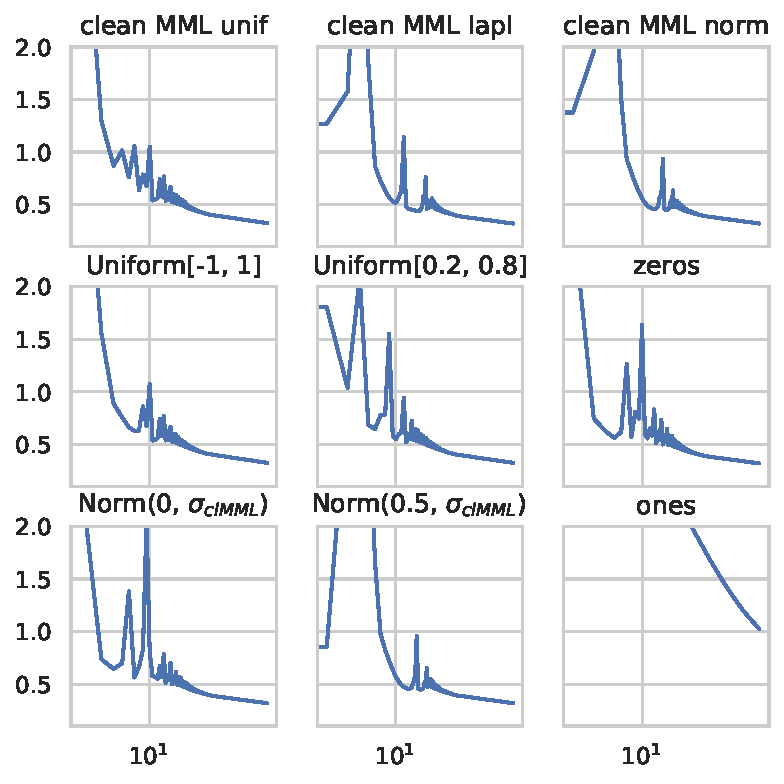
\includegraphics[width=1\linewidth]{pics/init_weights_loss.pdf}
%         \label{fig:init_weights_loss}
%      \end{subfigure}
%      \label{fig:init_weights_stats}
% \end{figure}

\begin{itemize}
    \item Инициализация единицами дала худший результат. Метод не успел проделать большой <<путь>> от единиц до нуля, вокруг которого должны концентрироваться веса модели.
    \item Инициализация $\U[0.2,0.8]$ дала немного меньшую точность, чем инициализация $\U[-1,1]$. Это тоже объясняется тем, что в первом случае метод должен проделать больший <<путь>> до нуля.
    \item Аналогично с $\N(0,\sigma_\text{clMML})$ и $\N(0.5,\sigma_\text{clMML})$.
    \item Инициализация нулями показала результат, совпадающий с инициализацией \texttt{clean MML norm}. Значит, инициализация теоретическим средним значением весов -- хорошая эвристика.
\end{itemize}

\subsection{Шаг и размер батча стохастического градиентного спуска.}

Эксперимент \ref{sec:gd_step} был повторен для метода стохастического градиентного спуска. Кроме $\alpha$ и $\beta$ исследовалась зависимость от размера батча. Результаты представлены на рис. \ref{fig:step_batch_rough}.

\begin{figure}[!htb]
     \caption{Точность моделей на валидационной выборке (по вертикали) в зависимости от эпохи стохастического градиентного спуска (по горизонтали).}
     \centering
     \begin{subfigure}[t]{0.493\linewidth}
        \caption{Accuracy}
        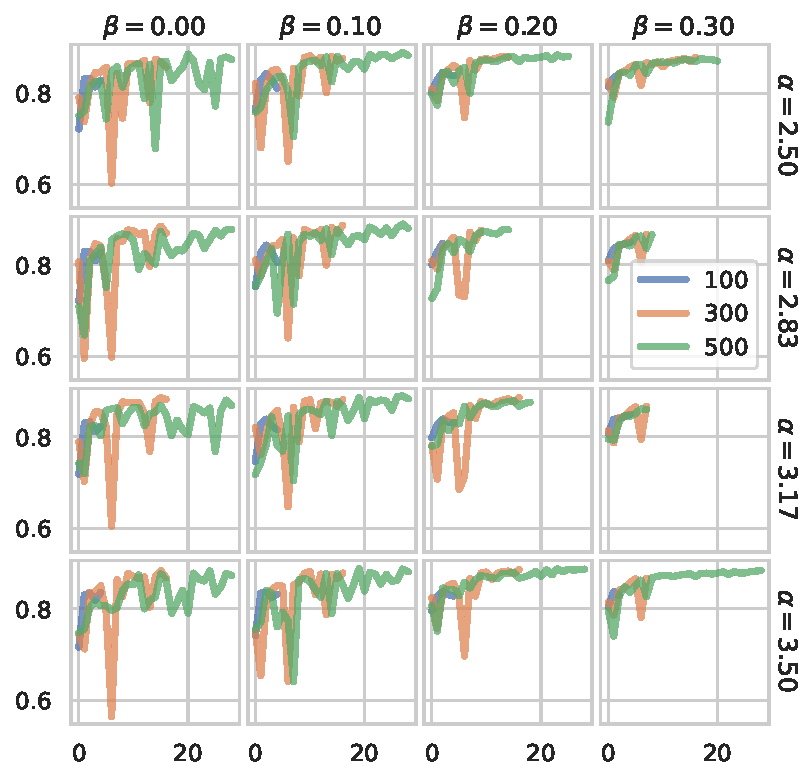
\includegraphics[width=1\linewidth]{pics/accur_step_batch.pdf}
        \label{fig:accur_step_batch}
     \end{subfigure}
     \begin{subfigure}[t]{0.48\linewidth}
        \centering
        \caption{Loss (лог. шкала по горизонтальной оси).}
        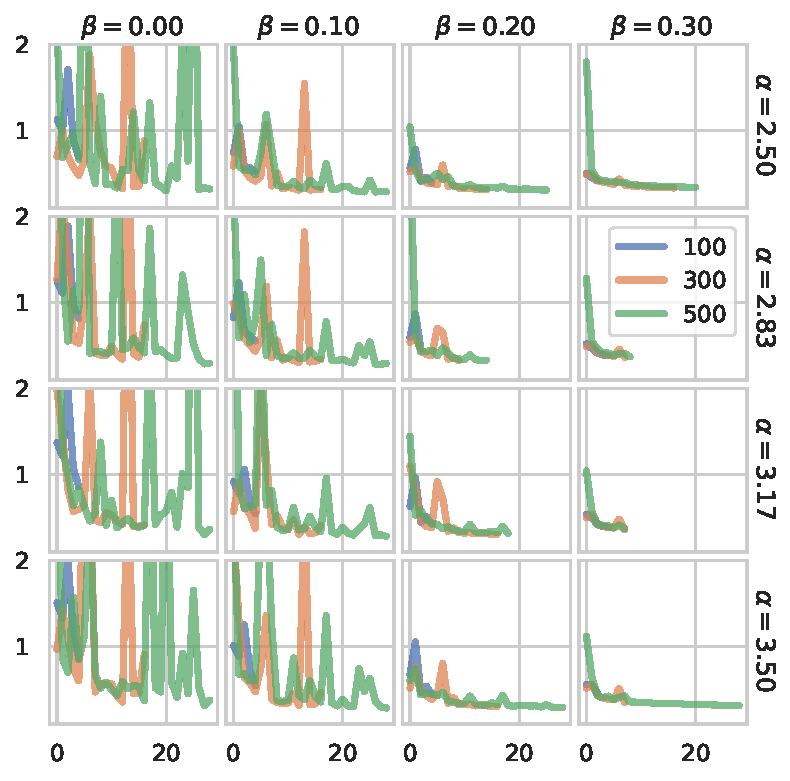
\includegraphics[width=1\linewidth]{pics/loss_step_batch.pdf}
        \label{fig:loss_step_batch}
     \end{subfigure}
     \label{fig:step_batch_rough}
\end{figure}

Видим ту же тенденцию с $\alpha,\ \beta$: их оптимальная пара способна достичь компромисс между осцилляциями и точностью. Заметим, что чем больше размер батча, тем большей точности методу удаётся достичь. Это объясняется тем, что с увеличением размера батча градиент, считаемый на каждой итерации, даёт более точную оценку градиента. В качестве компромисса между точностью и скоростью подсчёта будем использовать размер батча, равный 500.

\subsection{Начальное значение для стохастического градиентного спуска.}

Эксперимент \ref{sec:w0} был повторен для метода стохастического градиентного спуска. Оценки максимального правдоподобия не подсчитаны заново, а взяты прежние. Результаты предтавлены на рисунке

\begin{figure}[!htb]
     \caption{Точность моделей на валидационной выборке (по вертикали) в зависимости от шага стохастического градиентного спуска (по горизонтали). Демонстрация зависимости скорости сходимости градиентного спуска от начального значения.}
     \centering
     \begin{subfigure}[t]{0.48\linewidth}
        \caption{Accuracy}
        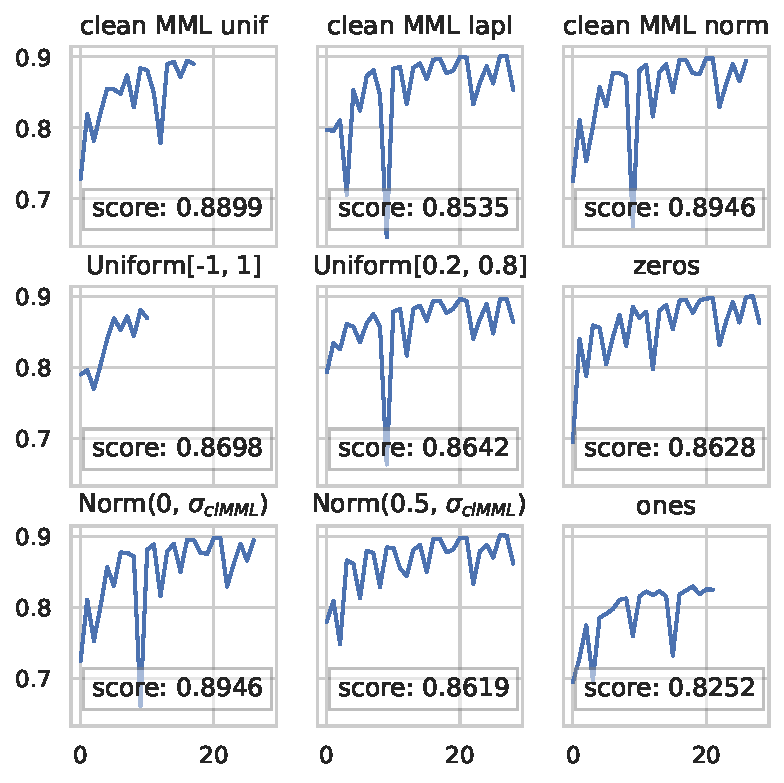
\includegraphics[width=1\linewidth]{pics/sgd_init_weights.pdf}
        \label{fig:sgd_init_weights}
     \end{subfigure}
     \begin{subfigure}[t]{0.48\linewidth}
        \centering
        \caption{Loss.}
        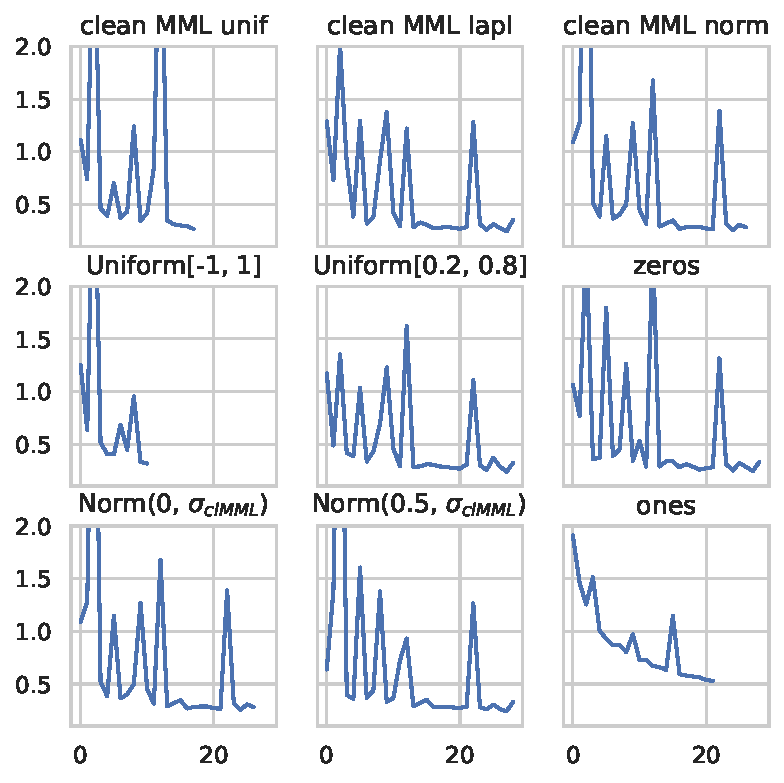
\includegraphics[width=1\linewidth]{pics/sgd_init_weights_loss.pdf}
        \label{fig:sgd_init_weights_loss}
     \end{subfigure}
     \label{fig:init_weights_stoch}
\end{figure}

Все результаты аналогичны результатам \ref{sec:w0}, за исключением того, что метод \texttt{zeros} дал меньшую точность, чем $\U[-1,1]$; метод $\N(0,\sigma_\text{clMML})$ дал большую точность, чем \texttt{clean MML lapl}.

\subsection{Сравнение GD и SGD.}

Методы GD и SGD были обучены с оптимальными параметрами $\alpha,\beta$ и batch size (рис. \ref{fig:gd_sgd}). Accuracy на валидационной выборке в методе SGD имеет такой же тренд, как и в методе GD. Отличие в том, что изменение происходит немонотонно, со <<скачками>>. Loss на обучающей выборке тоже отличается тем, что совершает <<скачки>>. Достигнутая точность SGD оказывается больше, чем точность GD.

\begin{figure}[!htb]
    \centering
    \caption{Сравнение методов GD и SGD. Зависимость accuracy и loss от номера итерации спуска.}
    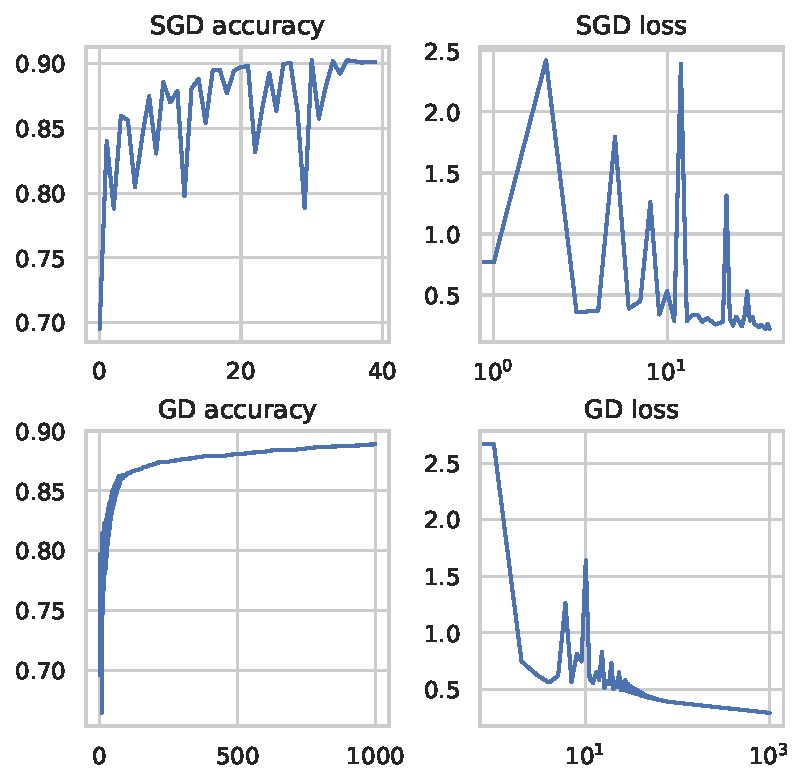
\includegraphics[width=0.6\linewidth]{pics/gd_sgd.pdf}
    \label{fig:gd_sgd}
\end{figure}

Заметим, что оптимальные параметры для GD отличаются от оптимальных параметров для SGD: $\alpha_\text{SGD}>\alpha_\text{GD}$ и $\beta_\text{SGD}<\beta_\text{GD}$. Также для метода SGD использовалось ограничение в 1500 итераций, а для GD -- в 1000. 

\subsection{Предобработка корпуса.}

С помощью {\texttt{nltk.corpus.stopwords.words('english')}~\cite{nltkstop}} были уделены стоп слова. Применена процедура лемматизации. Результаты приведены на рис. \ref{fig:nlp}. 

\begin{figure}[!htb]
     \caption{Результаты предобработки корпуса.}
     \centering
     \begin{subfigure}[t]{0.48\linewidth}
        \caption{Accuracy}
        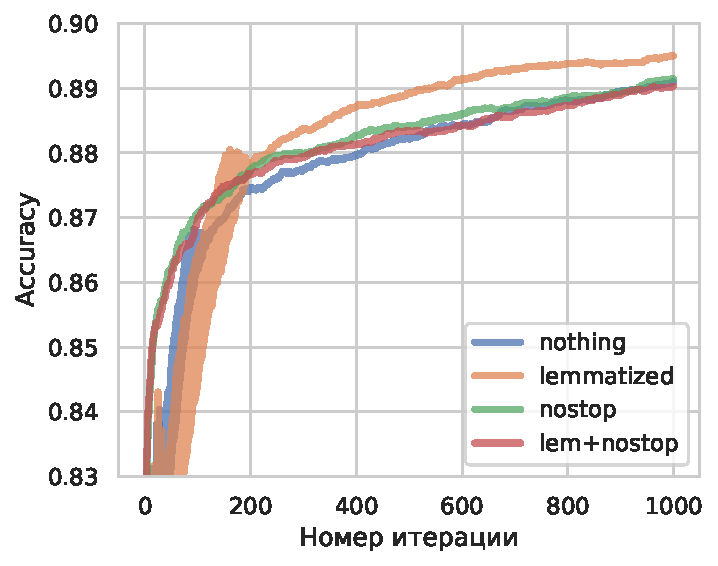
\includegraphics[width=1\linewidth]{pics/nlp_stuff.pdf}
        \label{fig:nl_stuff}
     \end{subfigure}
     \begin{subfigure}[t]{0.5\linewidth}
        \centering
        \caption{Время одной итерации.}
        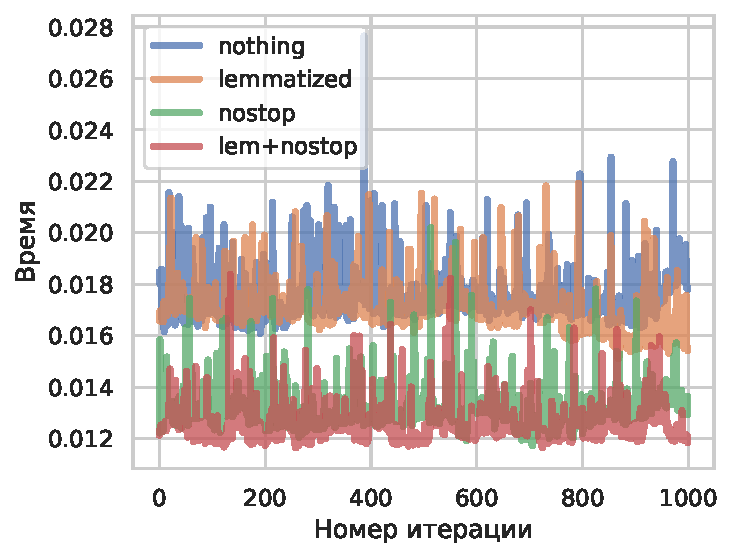
\includegraphics[width=1\linewidth]{pics/nlp_stuff_time.pdf}
        \label{fig:nl_stuff_time}
     \end{subfigure}
     \label{fig:nlp}
\end{figure}

Наибольшую точность дала процедура лемматизации \ref{fig:nl_stuff}. Причём удаление стоп слов из лемматизированного текста понизило качество. Значит, токсичность комментария сильно зависит от них. 

Сокращение признакового пространства (табл. \ref{tbl:feat_num}) отразилось на времени подсчёта каждой итерации (рис. \ref{fig:nl_stuff_time}). Чем меньше признаков, тем быстрее.

% \begin{table}[!hbt]
%     \centering
%     \begin{tabular}{l|c}
%         Метод & Число признаков \\
%         \hline
%         \texttt{nothing} & 15948 \\    
%         \texttt{lemmatized} & 12992  \\
%         \texttt{nostop} & 15805 \\
%         \texttt{lem+nostop} & 12862
%     \end{tabular}
%     \begin{tabular}{c|c|c}
%         Число признаков & Время \texttt{BoW} & Время \texttt{Tf-Idf} \\
%         \hline
%         12992 & 20.6 & 13.1 \\
%         3186 & 13.7 & 12.7 \\
%         558 & 14.1 & 9.5 \\
%         58 & 8.6 & 4.0
%     \end{tabular}
    
% \end{table}

\begin{figure}
\begin{floatrow}
\floatbox{table}[.3\textwidth][\FBheight][t]
{\caption{Сокращение.}
\label{tbl:feat_num}}
{\begin{tabular}{l|c}
        Метод & Число признаков \\
        \hline
        \texttt{nothing} & 15948 \\    
        \texttt{lemmatized} & 12992  \\
        \texttt{nostop} & 15805 \\
        \texttt{lem+nostop} & 12862
    \end{tabular}}\hspace*{1cm}
%
\floatbox{table}[.55\textwidth][\FBheight][t]
{\caption{Время счета в секундах.}
 \label{fig:time_vect}}
{\begin{tabular}{c|c|c}
        Число признаков & Время \texttt{BoW} & Время \texttt{Tf-Idf} \\
        \hline
        12992 & 20.6 & 13.1 \\
        3186 & 13.7 & 12.7 \\
        558 & 14.1 & 9.5 \\
        58 & 8.6 & 4.0
    \end{tabular}}
\end{floatrow}
\end{figure}



\subsection{Векторизация Tf-Idf.}

Модель была обучена методом GD с параметрами $\alpha=2.21,\ \beta=0.1$ на двух версиях векторизации исходного текста: \texttt{Bag of Words} и \texttt{Tf-Idf}. С помощью параметра \texttt{min\_df}~\cite{mindf} изменялось число используемых признаков. Результаты представлены на рис. \ref{fig:tfidf_bow}. 

\begin{figure}[!htb]
    \centering
    \caption{Кривая обучения в зависимости от числа признаков}
    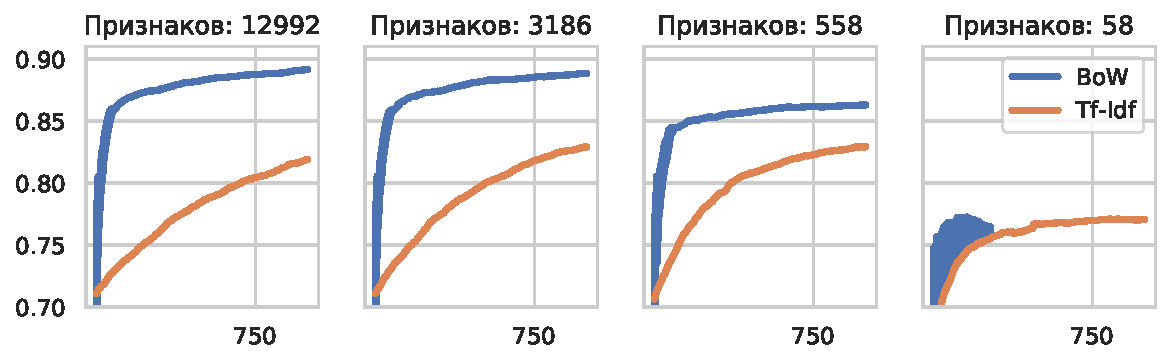
\includegraphics[width=0.85\linewidth]{pics/tfidf_bow.pdf}
    \label{fig:tfidf_bow}
\end{figure}

Векторизация \texttt{Tf-Idf} даёт меньшую точность. Это объяснимо тем, что для определения токсичности данного комментария необязательно учитывать все комментарии, как это делает \texttt{Tf-Idf}. Зависимость времени выполнения от числа признаков представлена в табл.

\subsection{Оптимальный шаг GD.}

\begin{wrapfigure}[15]{r}{0.5\linewidth}
    \centering
    \vspace{-7mm}
    \caption{Accuracy в зависимости от шага GD.}
    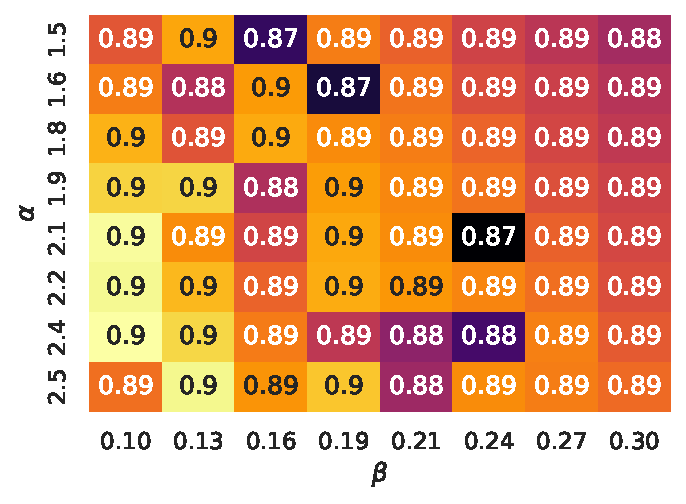
\includegraphics[width=1\linewidth]{pics/accur_step.pdf}
    \vspace{-8mm}
    \label{fig:accur_step}
\end{wrapfigure}
Логистическая регрессия была обучена методом GD сетке параметров $\alpha$ и $\beta$. На рис. \ref{fig:accur_step} представлены accuracy на валидационной выборке, которые в итоге удалось достичь. Ясно видна структура: к левому нижнему углу карты увеличивается accuracy, но в самом углу для некоторых моделей accuracy сильно низок. Это связано с ранее подмеченным наблюдением: при большом $\alpha$ и малом $\beta$ метод осциллирует, поэтому финальная точность может быть какой угодно. Так что искать оптимальные параметры стоит в окрестности карты, где нет таких выбросов.

Рассмотрим окрестность карты $\alpha\in[1.5, 1.93]$, $\beta\in[0.21, 0.3]$. Она отделена от выбросов. Соответствующие ей модели не осциллириуют и не <<застревают>>.

Поэтому оптимальными параметрами градиентного спуска будут $\alpha=1.93,\ \beta=0.21$, так как они обеспечивают компромисс между стабильностью сходимости и точностью.

% \begin{figure}[!htb]
%      \caption{Точность <<стабильных>> моделей на валидационной выборке (по вертикали) в зависимости от шага градиентного спуска (по горизонтали).}
%      \centering
%      \begin{subfigure}[t]{0.5\linewidth}
%         \caption{Accuracy}
%         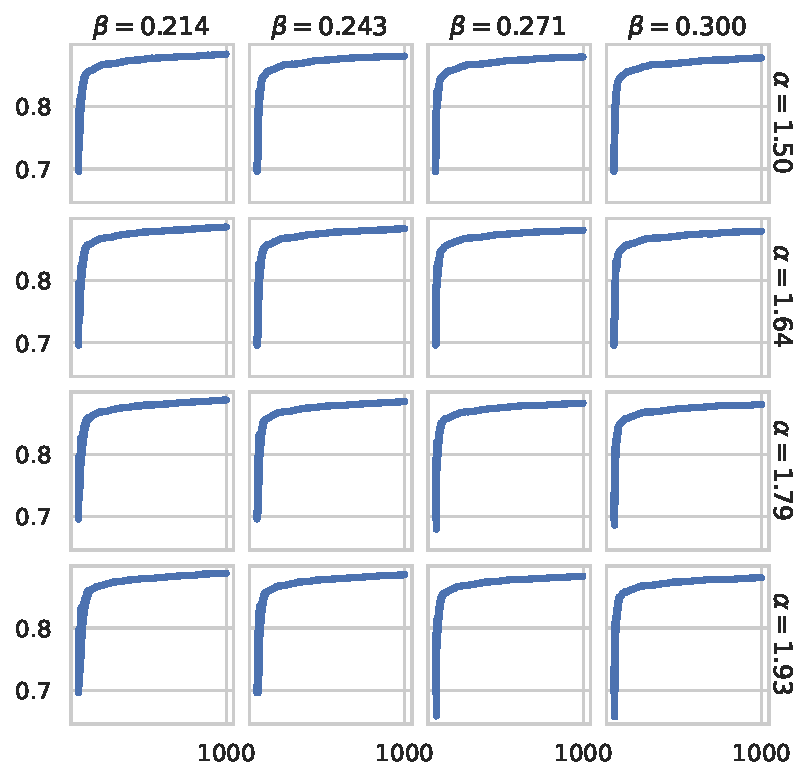
\includegraphics[width=1\linewidth]{pics/accur_step_best.pdf}
%         \label{fig:accur_step_best}
%      \end{subfigure}
%      \begin{subfigure}[t]{0.48\linewidth}
%         \centering
%         \caption{Loss (лог. шкала по горизонтальной оси).}
%         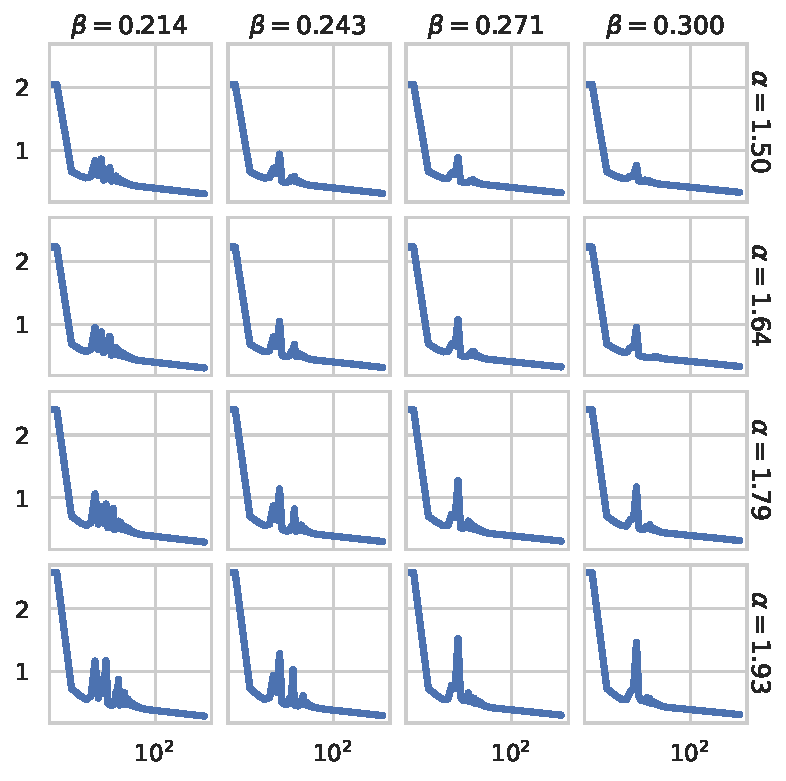
\includegraphics[width=1\linewidth]{pics/loss_step_best.pdf}
%         \label{fig:loss_step_best}
%      \end{subfigure}
%      \label{fig:step_best}
% \end{figure}

\subsection{Оптимальный шаг SGD.}

\begin{wrapfigure}[13]{r}{0.5\linewidth}
\centering
    \vspace{-12mm}
    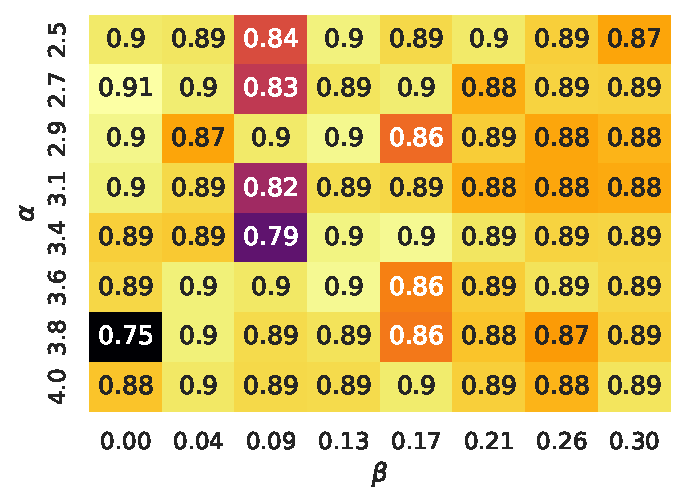
\includegraphics[width=1\linewidth]{pics/accur_step_stoch.pdf}
    \vspace{-8mm}
    \caption{Accuracy в зависимости от шага SGD.}
    \label{fig:accur_step_stoch}
\end{wrapfigure}
Модель логистической регрессии была обучена методом SGD на сетке параметров $\alpha$ и $\beta$ при batch size, равным 500. На рисунке \ref{fig:accur_step_stoch} представлена зависимость accuracy от параметров шага. На данной карте повторяется тенденция, которая была в случае GD: чем больше $\alpha$ и меньше $\beta$, тем <<нестабильнее>> сходимость. Окрестностью, компромиссной относительно выбросов и точности, является $\alpha\in[3.6, 4.0],\ \beta\in[0.04, 0.13]$. 
% Соответствующие accuracy и loss при обучении представлены на рисунке \ref{fig:step_batch_best}.

% \begin{figure}[!htb]
%      \caption{Точность выбранных моделей на валидационной выборке (по вертикали) в зависимости от эпохи стохастического градиентного спуска (по горизонтали).}
%      \centering
%      \begin{subfigure}[t]{0.493\linewidth}
%         \caption{Accuracy}
%         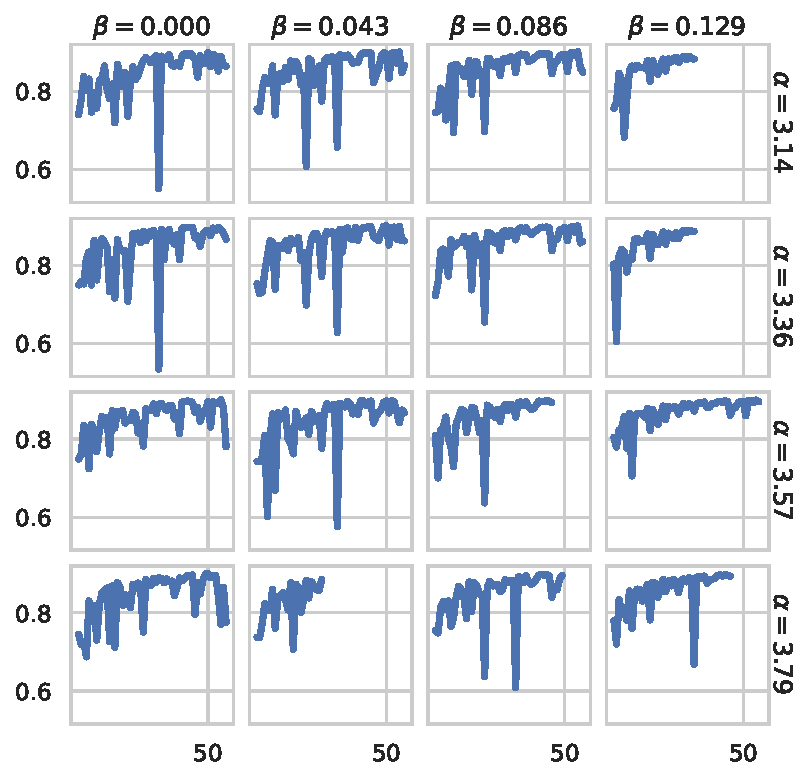
\includegraphics[width=1\linewidth]{pics/accur_step_best_stoch.pdf}
%         \label{fig:accur_step_best_stoch}
%      \end{subfigure}
%      \begin{subfigure}[t]{0.48\linewidth}
%         \centering
%         \caption{Loss (лог. шкала по горизонтальной оси).}
%         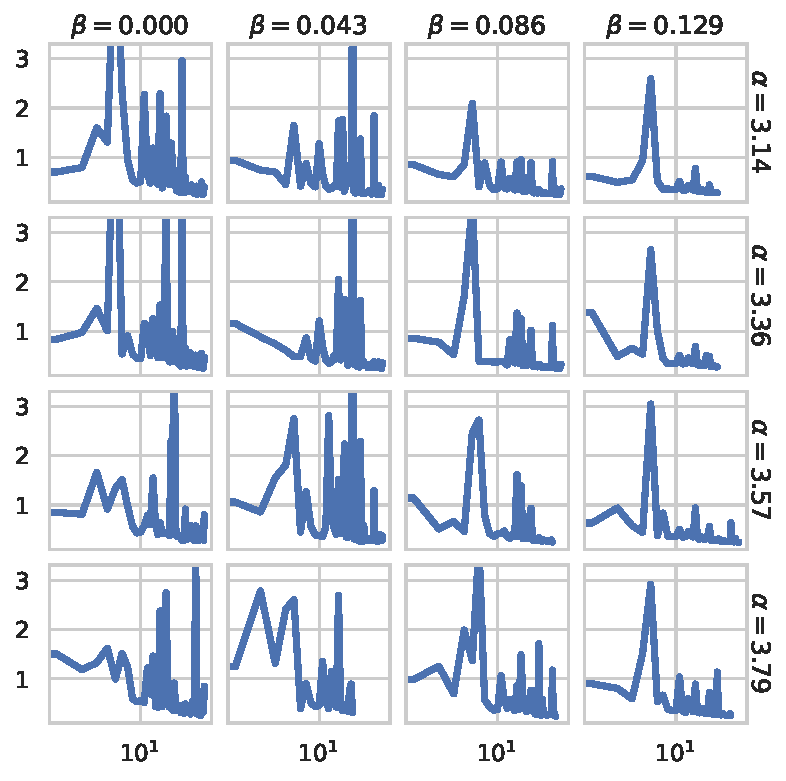
\includegraphics[width=1\linewidth]{pics/loss_step_best_stoch.pdf}
%         \label{fig:loss_step_best_stoch}
%      \end{subfigure}
%      \label{fig:step_batch_best}
% \end{figure}

В качестве оптимальных параметров SGD выберем $\alpha=3.79,\ \beta=0.13$.

\subsection{Контроль качества.}

С помощью модели логистической регрессии, обученной методом GD с оптимальными параметрами, были даны предсказания для тестовой выборки. Accuracy составила $0.8549$.

Если взять элементы с максимальным отступом (т.е. те, в ответах к которым модель уверена больше всего), то нетоксичные комментарии содержат благодарности и нейтральные слова о комментируемом материале, а токсичные комментарии по большей части состоят из ругательств.

Что характерно для ошибок false positive:
\begin{itemize}
    \item Слова kill, hate, которые употреблены не в отношении человека. Они необходимы в данном контесте: <<black mamba it is ponious snake of the word and but it not kills many people but king cobra kills many people in india>>. 
    \item Есть комментарий на тему истории одного ругательного слова. Это слово повторяется много раз.
    \item Очевидно, слово \texttt{slavery} окрашено негативно. Пример: <<islam and slavery is wikipedia articles for deletion islam and slavery would you care to vote thx>>.
    \item Некоторые, кажется, произошли из-за ошибок при составлении датасета: <<hello everyone i m just here to tell you that you re all freaks>>. Либо алгоритм смог распознать в этом шутку, а не оскорбление.
    \item Слово \texttt{nazi} с точки зрения модели имеет яркий негативный окрас.
    \item Некоторые слова имеют двойной смысл, один из них окрашен негативно. Например, <<you guys are sick>> помечено негативно, хотя чаще всего такую фразу употребляют, чтобы похвалить и выразить крайний восторг.
\end{itemize}

Ошибки false negative:
\begin{itemize}
    \item Пользователи писали ругательства с парой пропущенных букв, искажая слово каким-то уникальным способом. 
    \item Алгоритм не может распознать нераспространённые ругательства.
    \item Некоторые комментарии не кажутся токсичными, а просто выражают недовольство тем, как плохо сделана работа, которую они комментируют.
    \item Много нейтральных слов плюс несколько нелицеприятных или имеющих двойной смысл -- верный способ получить ошибку false negative.
\end{itemize}

\section{Выводы.}

Градиентные методы GD и SGD чувствительны к выбору шага (learning rate) и начальному значению $w_0$. Если шаг будет слишком большим, то метод будет осциллировать вокруг оптимума. Если шаг будет слишком быстро угасать или начальное значение будет далеко от оптимума, то метод может <<не добраться>> до него. Оптимальный шаг должен достичь компромисс между осцилляциями и точностью.

Метод SGD дополнительно чувствителен к размеру батча. Чем он меньше, тем грубее используемая на каждой итерации оценка градиента и тем медленнее и с большими осцилляциями сходится метод. В целом, он менее устойчив в сравнении с GD и требует более точной настройки параметров.

Время работы обоих методов зависит от размера признакового пространства и размеров обрабатываемых датасетов.

\newpage
\printbibliography

\end{document}
